\subsection{Correlated Private Randomness}
\begin{frame}{Correlated Private Randomness (Correlation)}
\begin{figure}
\begin{center}
\begin{tikzpicture}[every node/.style={minimum width=1cm}]
\node [alice] (alice) {};
\node[bob, right=5cm of alice,  mirrored] (bob){};
%\draw[->, thick] (alice) -- coordinate[near start] (aux) (bob);
\node[draw, ellipse, above right=1.3cm of alice, thick] (dealer) {$ (r_A, r_B) \sim (R_A, R_B) $}; 
\draw[->, thick] (dealer)--(alice) node[midway,left]{$ r_A $};
\draw[->, thick] (dealer)--(bob) node [midway, right] {$ r_B $};
\draw[dashed, thick] ($(alice.south west) + (0,-0.2)$) -- ($(bob.south east)+(0,-0.2)$);
\draw [->, thick ] ($(alice.south) + (1, -0.5)$) -- ($(bob.south) + (-1, -0.5)$);
\draw [<-, thick ] ($(alice.south) + (1, -1)$) -- ($(bob.south) + (-1, -1)$) node [midway, below] (dots) {$ \vdots $};
\draw [->, thick ] ($(alice.south) + (1, -2)$) -- ($(bob.south) + (-1, -2)$);

\node[fit=(alice)(bob)(dealer)] (help1){};
\node[left=of help1, align=center] (off) {Preprocessing \\ Phase};

\node[align=center] (on) at (off|-dots.north) {Online \\ Phase};
\end{tikzpicture}
\end{center}
\end{figure}


\onslide<3->{\setbeamercolor{block title}{bg=gray, fg=white}
\begin{block}{Notes}
	\begin{itemize}
		\item  The preprocessing phase is independent of the functionality or the inputs fed to the functionality by the parties.
		\item Secret shares $(r_A, r_B)  $ are vulnerable to leakage attacks.
	\end{itemize}
\end{block}}

%	\begin{itemize}
%		\item A fundamental cryptographic resource for computing securely over private data
%		\item Offline prepocessing phase: generates correlated {\em private shares} $ (r_A, r_B) \sim (R_A, R_B) $, provides $r_A$ to Alice and $r_B$ to Bob 
%		%\item Online phase: uses the shares to securely compute intended functionality
%		\item Secret shares vulnerable to leakage attacks
%		\item  A graph-theoretic representation of correlation: a weighted bipartite graph $  G = (L, R, E) $
		
%		\begin{itemize}
%	  		\item $ L $: the set of all possible private shares $ r_A $ for Alice
%	  		\item $ R $: the set of all possible private shares $ r_B $ for Bob
%			\item Weight of the edge $ (r_A, r_B) $ is  $ p(r_A, r_B) $
%		\end{itemize}
%	\end{itemize}
\end{frame}


%\begin{frame}{Correlation (Examples)}
%	\begin{figure}[htp] \footnotesize
\begin{center}
\begin{tikzpicture}[
vert/.style = {node distance = 5mm, circle, draw, fill = purdue-gold!40, thick, inner sep = 1pt},  
bdd/.style = {rectangle, draw, inner sep = 5mm}, 
cc/.style = {rounded corners = 5pt, fill = black!50, pattern = crosshatch dots, pattern color = gray}, 
minimum size = 5mm,
]
%[
%vert/.style = {node distance = 5mm, circle, draw, fill = black!10, thick, inner sep = 1pt},  
%bdd/.style = {rectangle, draw, inner sep = 5mm}, 
%cc/.style = {rounded corners = 5pt, fill = black!50, pattern = crosshatch dots, pattern color = gray}, 
%minimum size = 5mm,
%]

%%% 
\node at (0,0) (l1) {L};
\node [vert, below = of l1] (c00)  {}; 
\node [vert, below = of c00] (c01) {$r_A$}; 
\node [vert, below = of c01] (c10) {}; 
%\node [vert, below = of c10] (c11) {11}; 

\node [node distance = 15mm, right = of l1] (r1) {R};
\node [vert, below = of r1] (d00) {}; 
\node [vert, below = of d00] (d01) {$ r_B $}; 
\node [vert, below = of d01] (d10) {}; 
%\node [vert, below = of d10] (d11) {11};

\draw [thick] (c01) -- (d01) node [midway, above] {$ p(r_A, r_B) $};

\coordinate (temp) at ($0.5*(c10)+0.5*(d10)$);
\node[node distance = 1 cm, below of = temp] {\underline{Graph of General Correlation}}; 

%\pause 

%%% ROT
%\node [node distance = 1cm, right = of r1] (l2) {$ (x_0, x_1) $};
%\node [vert, below = of l2] (a00) {00}; 
%\node [vert, below = of a00] (a01) {01}; 
%\node [vert, below = of a01] (a10) {10}; 
%\node [vert, below = of a10] (a11) {11}; 
%
%\node [right = of l2] (r2) {$(b, x_b)$};
%\node [vert, below = of r2] (b00) {00}; 
%\node [vert, below = of b00] (b01) {01}; 
%\node [vert, below = of b01] (b10) {10}; 
%\node [vert, below = of b10] (b11) {11}; 
%
%\draw (a00) -- (b00) (a00) -- (b10); 
%\draw (a01) -- (b00) (a01) -- (b11); 
%\draw (a10) -- (b01) (a10) -- (b10); 
%\draw (a11) -- (b01) (a11) -- (b11); 
%
%\coordinate (temp) at ($0.5*(a11)+0.5*(b11)$);
%\node[below of = temp] {\underline{Random Oblivious Transfer}}; 

%\pause 

%% IP
%%% First Correlation 
%\node [node distance = 3cm, right = of r1] {$ \pred{IP} $};

\node [vert, node distance = 3cm, right = of b00] (e00) {00}; 
\node [vert, below = of e00] (e01) {01}; 
\node [vert, below = of e01] (e10) {10}; 
\node [vert, below = of e10] (e11) {11}; 

\node [vert, node distance = 15mm, right = of e00] (f00) {00}; 
\node [vert, below = of f00] (f01) {01}; 
\node [vert, below = of f01] (f10) {10}; 
\node [vert, below = of f10] (f11) {11}; 


\draw [thick] (e00) -- (f00)  (e00) -- (f01)  (e00) -- (f10)  (e00) -- (f11); 
\draw [thick] (e01) -- (f00)  (e01) -- (f10); 
\draw [thick] (e10) -- (f00)  (e10) -- (f01); 
\draw [thick] (e11) -- (f00)  (e11) -- (f11);

\coordinate (temp) at ($0.5*(e11)+0.5*(f11)$);
\node[below of = temp, align=center] {\underline{$ \IP[\GF{2}^2] $}}; 


\end{tikzpicture}
%\caption{Some representative examples of a correlation}
\end{center}
\end{figure}

%\end{frame}
		
\subsection{Oblivious Transfer}
\begin{frame}{Oblivious Transfer (\OT)}
	\begin{figure}
		\begin{center}
			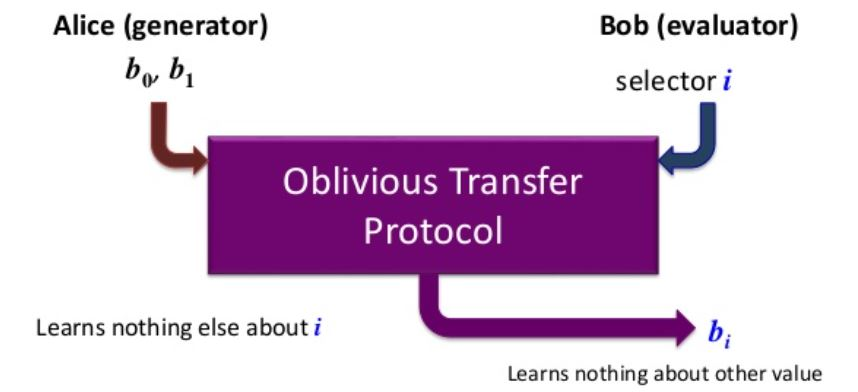
\includegraphics[scale = 0.5]{OT-1}
		\end{center}
	\caption{1-out-of-2 \OT}
	\end{figure}
	
	\pause
	
	\begin{definition}[Random Oblivious Transfer (\ROT)]
	\begin{itemize}
		\item a randomized version of \OT
		\item samples $ x_0, x_1, b  $ independently and uniformly at random 
		\item provides secret shares $ (x_0, x_1) $ to Alice and $ (b, x_b) $ to Bob
	\end{itemize}
	\end{definition}
 	%\tiny \footfullcite{https://www.slideshare.net/DavidEvansUVa/darmstadt-48999286}
\end{frame}

\subsection{Correlation Extractor}
\begin{frame}{Correlation Extractor (CorrExt)}
	\begin{itemize}
		\item Introduced by Ishai, Kushilevitz, Ostrovsky, and Sahai at FOCS 2009 \cite{FOCS:IKOS09} to address leakage attacks. 
		\item Takes leaky correlations as input and produces secure independent
		copies of oblivious transfer (OT)
		\pause
		\begin{definition}[Correlation Extractor (CorrExt)]
			A $ (n,m,t,\epsilon) $-CorrExt for $ (R_A, R_B) $: 
			\begin{itemize}
				\item Is a two-party interactive protocol	
				\item Takes \underline{$n$-bit secret shares} $ (r_A, r_B) \sim (R_A, R_B) $ as input
				\item Produces \underline{$ m $ independent OT's}
				\item Allows \underline{$ t $-bits of leakage} on the secret share
				\item Secures against semi-honest adversaries with \underline{simulation error $ \epsilon $}
			\end{itemize}
		\end{definition}
		%
		%		\item Criteria for a good correlation extractor:
		%\begin{itemize}
		%	\item Number of OTs produced $ (m) $
		%	\item Number of leakage bits $ (t) $
		%	\item Simulation error $ (\epsilon) $
		%	\item Round complexity of protocol $ (\#) $
		%\end{itemize}
		\pause
		\item A direct analog of privacy amplification and randomness extractor
		\item But ensure security against insider attacks
	\end{itemize}
\end{frame}
	
	%\input{fig-example1}

%\begin{frame}{Introduction (Examples)}
	%\input{fig-example1}
%\end{frame}
